\chapter{Naměřená výkonnostní data}

\begin{table}[htbp]
    \caption{\textbf{AMD Ryzen 4000 5}. Procesor byl omezen na 3 hodinové rychlosti (sloupce), přičemž jednotlivé řádky reprezentují průměrný násobek ideální rychlosti 100 naměřených snímků (tedy bylo naměřeno celkem 1000 konzistentních snímku specifické hry a okno po 10 snímcích bylo zprůměrováno). Pokračování tabulky \ref{amd-ryzen-perf-2}}
    \begin{center}
    \begin{tabular}{ |c|c|c|c|c|c| }
     \hline
     \textbf{1x/1.4GHz} & \textbf{2x/1.4GHz} & \textbf{1x/1.7GHz} & \textbf{2x/1.7MHz} & \textbf{1x/3GHz} & \textbf{2x/3MHz} \\
     \hline
        0.967953 & 0.660651 & 1.177842 & 0.802855 & 2.753748 & 1.866711 \\
        1.021956 & 0.714269 & 1.245324 & 0.867937 & 2.907587 & 2.028165 \\
        0.952063 & 0.608470 & 1.157768 & 0.766193 & 2.698310 & 1.796814 \\
        1.013590 & 0.691830 & 1.220589 & 0.844670 & 2.861357 & 1.964868 \\
        0.949956 & 0.626657 & 1.146902 & 0.763004 & 2.679373 & 1.776648 \\
        0.998788 & 0.692615 & 1.217571 & 0.844600 & 2.841532 & 1.976229 \\
        0.950634 & 0.626210 & 1.149305 & 0.764787 & 2.649055 & 1.770648 \\
        1.011210 & 0.691721 & 1.220672 & 0.841403 & 2.829500 & 1.968275 \\
        0.948727 & 0.627635 & 1.140178 & 0.762465 & 2.685867 & 1.787347 \\
        1.009227 & 0.691611 & 1.227207 & 0.840232 & 2.852648 & 1.968768 \\
        0.947913 & 0.624947 & 1.153232 & 0.757096 & 2.686585 & 1.776579 \\
        1.009133 & 0.691848 & 1.228513 & 0.839240 & 2.872848 & 1.962725 \\
        0.949992 & 0.623523 & 1.154841 & 0.761236 & 2.660109 & 1.763244 \\
        1.012998 & 0.662046 & 1.231141 & 0.839299 & 2.858463 & 1.974491 \\
        0.944989 & 0.622910 & 1.147994 & 0.758766 & 2.675943 & 1.771073 \\
        1.009707 & 0.692042 & 1.228346 & 0.839692 & 2.846368 & 1.966736 \\
        0.948496 & 0.625481 & 1.150522 & 0.762029 & 2.680474 & 1.780018 \\
        1.020564 & 0.698591 & 1.233510 & 0.845116 & 2.875341 & 1.974169 \\
        0.955350 & 0.630879 & 1.159687 & 0.765969 & 2.705843 & 1.781338 \\
        1.016089 & 0.692792 & 1.229790 & 0.845268 & 2.861546 & 1.967983 \\
        0.953212 & 0.626627 & 1.157796 & 0.761806 & 2.718002 & 1.780613 \\
        1.012300 & 0.692556 & 1.225741 & 0.838726 & 2.885216 & 1.950384 \\
        0.951137 & 0.626784 & 1.158032 & 0.761489 & 2.713928 & 1.766997 \\
        1.013305 & 0.692123 & 1.225749 & 0.846733 & 2.895792 & 1.964867 \\
        0.954652 & 0.628600 & 1.164545 & 0.762959 & 2.726558 & 1.779830 \\
        1.013413 & 0.691397 & 1.230657 & 0.843462 & 2.875053 & 1.956245 \\
        0.955127 & 0.627639 & 1.163608 & 0.767903 & 2.730391 & 1.781067 \\
        1.007080 & 0.690659 & 1.231025 & 0.842135 & 2.845124 & 1.948782 \\
        0.945962 & 0.627589 & 1.156600 & 0.763230 & 2.707818 & 1.768893 \\
        1.010141 & 0.691136 & 1.225642 & 0.840501 & 2.891845 & 1.967905 \\
        0.959790 & 0.634844 & 1.173308 & 0.772402 & 2.739660 & 1.789174 \\
        1.012774 & 0.694421 & 1.235905 & 0.840162 & 2.890630 & 1.958250 \\
        0.941036 & 0.629470 & 1.160307 & 0.756637 & 2.723393 & 1.785323 \\
        1.001889 & 0.693560 & 1.232101 & 0.841870 & 2.891902 & 1.962635 \\
        0.943416 & 0.628478 & 1.165127 & 0.763130 & 2.708328 & 1.776906 \\
        1.003956 & 0.694900 & 1.230676 & 0.838805 & 2.885710 & 1.960541 \\
        0.948227 & 0.628819 & 1.162590 & 0.762819 & 2.735948 & 1.779839 \\
        1.013143 & 0.693586 & 1.235372 & 0.841782 & 2.904402 & 1.974533 \\
        0.946525 & 0.629481 & 1.168492 & 0.765998 & 2.738970 & 1.782431 \\
        1.006079 & 0.693265 & 1.235775 & 0.838810 & 2.895302 & 1.959135 \\
        0.948796 & 0.630495 & 1.162529 & 0.768382 & 2.735157 & 1.780691 \\
        
     \hline
    \end{tabular}
    \end{center}
    \label{amd-ryzen-perf}
\end{table}

\begin{table}[htbp]
    \caption{\textbf{AMD Ryzen 4000 5}. Pokračování tabulky \ref{amd-ryzen-perf-3}}
    \begin{center}
    \begin{tabular}{ |c|c|c|c|c|c| }
     \hline
     \textbf{1x/1.4GHz} & \textbf{2x/1.4GHz} & \textbf{1x/1.7GHz} & \textbf{2x/1.7MHz} & \textbf{1x/3GHz} & \textbf{2x/3MHz} \\
     \hline
        1.014328 & 0.693983 & 1.237621 & 0.847253 & 2.892178 & 1.972136 \\
        0.953787 & 0.628826 & 1.164285 & 0.762520 & 2.732571 & 1.783905 \\
        1.014806 & 0.696550 & 1.234170 & 0.846648 & 2.868323 & 1.970332 \\
        0.956611 & 0.630253 & 1.166207 & 0.769802 & 2.725551 & 1.782815 \\
        1.012033 & 0.694975 & 1.237662 & 0.844254 & 2.898626 & 1.972057 \\
        0.950294 & 0.632380 & 1.164547 & 0.756961 & 2.731532 & 1.779316 \\
        0.993995 & 0.695041 & 1.233714 & 0.843916 & 2.894082 & 1.970537 \\
        0.941791 & 0.629128 & 1.157075 & 0.764911 & 2.728946 & 1.797333 \\
        1.002849 & 0.694999 & 1.235865 & 0.840646 & 2.891623 & 1.982617 \\
        0.953391 & 0.629880 & 1.163253 & 0.761694 & 2.722710 & 1.803316 \\
        1.007728 & 0.693358 & 1.236065 & 0.834506 & 2.902842 & 1.982162 \\
        0.942626 & 0.630388 & 1.163983 & 0.762922 & 2.730648 & 1.793742 \\
        1.002000 & 0.695992 & 1.232990 & 0.840201 & 2.891229 & 1.976936 \\
        0.933302 & 0.628536 & 1.163409 & 0.770808 & 2.736006 & 1.785235 \\
        1.009791 & 0.695957 & 1.236435 & 0.848073 & 2.899871 & 1.984652 \\
        0.941929 & 0.630641 & 1.167811 & 0.769895 & 2.734105 & 1.784323 \\
        1.007856 & 0.686512 & 1.235751 & 0.840594 & 2.900186 & 1.966735 \\
        0.953287 & 0.626911 & 1.163943 & 0.761610 & 2.726532 & 1.782491 \\
        1.010908 & 0.695153 & 1.234478 & 0.845754 & 2.850332 & 1.969029 \\
        0.944254 & 0.627254 & 1.156130 & 0.762630 & 2.711149 & 1.775234 \\
        1.008185 & 0.694801 & 1.232340 & 0.841005 & 2.881186 & 1.963256 \\
        0.946039 & 0.627757 & 1.158614 & 0.760605 & 2.703842 & 1.783541 \\
        1.007541 & 0.693260 & 1.228071 & 0.839275 & 2.880050 & 1.967225 \\
        0.944738 & 0.626835 & 1.154384 & 0.757040 & 2.697456 & 1.774669 \\
        1.006160 & 0.688294 & 1.232170 & 0.834484 & 2.872949 & 1.963367 \\
        0.943533 & 0.623836 & 1.154939 & 0.754709 & 2.660142 & 1.736704 \\
        1.006431 & 0.691562 & 1.229461 & 0.828565 & 2.872303 & 1.964661 \\
        0.946468 & 0.626684 & 1.159355 & 0.756633 & 2.713552 & 1.768796 \\
        1.004435 & 0.689071 & 1.227291 & 0.838136 & 2.868566 & 1.962128 \\
        0.934921 & 0.624844 & 1.153880 & 0.753633 & 2.699735 & 1.774327 \\
        1.008477 & 0.689401 & 1.230704 & 0.836536 & 2.880236 & 1.966218 \\
        0.944659 & 0.625872 & 1.150912 & 0.756944 & 2.705485 & 1.778557 \\
        1.015397 & 0.694705 & 1.241444 & 0.844660 & 2.903413 & 1.977742 \\
        0.950761 & 0.630638 & 1.165042 & 0.758740 & 2.715742 & 1.791366 \\
        1.007359 & 0.693223 & 1.233846 & 0.843092 & 2.880240 & 1.952200 \\
        0.944579 & 0.627403 & 1.160964 & 0.761233 & 2.721445 & 1.775152 \\
        1.010641 & 0.695013 & 1.229316 & 0.841263 & 2.891097 & 1.965340 \\
        0.947246 & 0.629885 & 1.158331 & 0.766671 & 2.718438 & 1.784515 \\
        1.015650 & 0.692720 & 1.239584 & 0.839329 & 2.898660 & 1.969109 \\
        0.946619 & 0.627706 & 1.161185 & 0.761933 & 2.723480 & 1.774710 \\
        1.004146 & 0.694073 & 1.234127 & 0.837957 & 2.881136 & 1.955137 \\
        0.946752 & 0.627905 & 1.164081 & 0.762125 & 2.698138 & 1.774320 \\
        1.005840 & 0.693069 & 1.230594 & 0.838697 & 2.879157 & 1.959552 \\
        0.946325 & 0.625101 & 1.157356 & 0.756876 & 2.703806 & 1.781619 \\
     \hline
    \end{tabular}
    \end{center}
    \label{amd-ryzen-perf-2}
\end{table}

\begin{table}[htbp]
    \caption{\textbf{AMD Ryzen 4000 5}.}
    \begin{center}
    \begin{tabular}{ |c|c|c|c|c|c| }
     \hline
     \textbf{1x/1.4GHz} & \textbf{2x/1.4GHz} & \textbf{1x/1.7GHz} & \textbf{2x/1.7MHz} & \textbf{1x/3GHz} & \textbf{2x/3MHz} \\
     \hline
        1.008899 & 0.692432 & 1.232953 & 0.841765 & 2.878013 & 1.950519 \\
        0.952455 & 0.629579 & 1.165142 & 0.762871 & 2.720674 & 1.780712 \\
        1.009791 & 0.694312 & 1.232626 & 0.834862 & 2.881935 & 1.956572 \\
        0.942759 & 0.628761 & 1.159043 & 0.762604 & 2.717130 & 1.782168 \\
        1.004613 & 0.692710 & 1.231671 & 0.840767 & 2.886271 & 1.964042 \\
        0.944875 & 0.631079 & 1.161551 & 0.764721 & 2.710477 & 1.783279 \\
        1.013529 & 0.695030 & 1.234849 & 0.842502 & 2.897147 & 1.966990 \\
        0.954270 & 0.629325 & 1.164827 & 0.764606 & 2.695506 & 1.793237 \\
        1.018024 & 0.693532 & 1.237851 & 0.840485 & 2.858340 & 1.979354 \\
        0.956625 & 0.629511 & 1.164275 & 0.766778 & 2.694798 & 1.797358 \\
        1.013077 & 0.693832 & 1.237927 & 0.842670 & 2.877039 & 1.973729 \\
        0.952169 & 0.627651 & 1.163873 & 0.767042 & 2.693091 & 1.792998 \\
        1.018078 & 0.696044 & 1.235108 & 0.847078 & 2.844889 & 1.983881 \\
        0.956209 & 0.630240 & 1.163153 & 0.768392 & 2.709724 & 1.793017 \\
        1.016369 & 0.693181 & 1.233023 & 0.846147 & 2.889254 & 1.981691 \\
     \hline
    \end{tabular}
    \end{center}
    \label{amd-ryzen-perf-3}
\end{table}

\begin{table}[htbp]
    \caption{\textbf{Intel i5 2520}. Procesor byl omezen na 3 hodinové rychlosti (sloupce), přičemž jednotlivé řádky reprezentují průměrný násobek ideální rychlosti 100 naměřených snímků (tedy bylo naměřeno celkem 1000 konzistentních snímku specifické hry a okno po 10 snímcích bylo zprůměrováno). Pokračování tabulky \ref{intel-perf-2}}
    \begin{center}
    \begin{tabular}{ |c|c|c|c|c|c| }
     \hline
     \textbf{1x/1.4GHz} & \textbf{2x/1.4GHz} & \textbf{1x/1.7GHz} & \textbf{2x/1.7MHz} & \textbf{1x/3GHz} & \textbf{2x/3MHz} \\
     \hline
        0.655273 & 0.454683 & 0.795157 & 0.548547 & 1.434706 & 0.980536 \\
        0.683726 & 0.488089 & 0.839157 & 0.582340 & 1.509348 & 1.050314 \\
        0.641811 & 0.436267 & 0.790519 & 0.525791 & 1.419877 & 0.936589 \\
        0.681576 & 0.476474 & 0.833991 & 0.580165 & 1.498776 & 1.020135 \\
        0.638984 & 0.433638 & 0.786628 & 0.525719 & 1.414686 & 0.932876 \\
        0.685392 & 0.475978 & 0.831502 & 0.574748 & 1.495392 & 1.026580 \\
        0.649344 & 0.433303 & 0.787209 & 0.526461 & 1.394714 & 0.936325 \\
        0.685921 & 0.477102 & 0.832138 & 0.577407 & 1.473665 & 1.029583 \\
        0.635652 & 0.431858 & 0.783851 & 0.524666 & 1.395248 & 0.936004 \\
        0.685154 & 0.475448 & 0.827906 & 0.560239 & 1.440413 & 1.026692 \\
        0.646601 & 0.431531 & 0.777453 & 0.525573 & 1.398668 & 0.928503 \\
        0.683128 & 0.470788 & 0.831443 & 0.578677 & 1.478543 & 1.022013 \\
        0.638645 & 0.429772 & 0.781060 & 0.524011 & 1.400219 & 0.935716 \\
        0.682870 & 0.473997 & 0.831219 & 0.577584 & 1.488241 & 1.029347 \\
        0.644370 & 0.431556 & 0.784476 & 0.520098 & 1.393303 & 0.935004 \\
        0.680888 & 0.468052 & 0.831552 & 0.577193 & 1.492435 & 1.023903 \\
        0.645353 & 0.432664 & 0.783018 & 0.526869 & 1.410299 & 0.937545 \\
        0.685205 & 0.474624 & 0.826400 & 0.581488 & 1.488719 & 1.030657 \\
        0.651709 & 0.435752 & 0.785407 & 0.530457 & 1.420636 & 0.943905 \\
        0.680046 & 0.475559 & 0.820479 & 0.579492 & 1.500238 & 1.019065 \\
        0.650415 & 0.434071 & 0.752909 & 0.529131 & 1.417208 & 0.938579 \\
        0.681644 & 0.477120 & 0.741728 & 0.580750 & 1.495146 & 1.029904 \\
        0.650511 & 0.434683 & 0.715668 & 0.529571 & 1.400238 & 0.939542 \\
        0.685131 & 0.476387 & 0.640797 & 0.580741 & 1.498681 & 1.030380 \\
        0.650571 & 0.435494 & 0.779751 & 0.519795 & 1.418142 & 0.939718 \\
        0.685456 & 0.476292 & 0.832266 & 0.580857 & 1.498149 & 1.030429 \\
        0.649010 & 0.434497 & 0.788545 & 0.529289 & 1.416607 & 0.939612 \\
        0.676332 & 0.476674 & 0.816672 & 0.567529 & 1.495711 & 1.030313 \\
        0.650121 & 0.435022 & 0.737253 & 0.525021 & 1.416910 & 0.936886 \\
        0.686493 & 0.470448 & 0.818027 & 0.580848 & 1.496875 & 1.028657 \\
        0.652188 & 0.435122 & 0.784727 & 0.530456 & 1.415484 & 0.941379 \\
        0.669511 & 0.473661 & 0.832576 & 0.580225 & 1.494753 & 1.030146 \\
        0.650381 & 0.433867 & 0.788396 & 0.528983 & 1.415243 & 0.936642 \\
        0.686862 & 0.473612 & 0.834614 & 0.580466 & 1.496939 & 1.029834 \\
        0.648732 & 0.429787 & 0.791603 & 0.526708 & 1.415177 & 0.940144 \\
        0.684949 & 0.477071 & 0.836047 & 0.580443 & 1.499680 & 1.030595 \\
        0.649732 & 0.434427 & 0.787357 & 0.530038 & 1.419447 & 0.938522 \\
        0.685849 & 0.476896 & 0.833103 & 0.572328 & 1.497756 & 1.030763 \\
        0.651100 & 0.434471 & 0.790977 & 0.530968 & 1.419590 & 0.940348 \\
        0.684771 & 0.476458 & 0.833666 & 0.580602 & 1.476317 & 1.030820 \\
        0.651248 & 0.433157 & 0.789950 & 0.530401 & 1.420123 & 0.940205 \\
     \hline
    \end{tabular}
    \end{center}
    \label{intel-perf}
\end{table}

\begin{table}[htbp]
    \caption{\textbf{Intel i5 2520}. Pokračování tabulky \ref{intel-perf-3}}
    \begin{center}
    \begin{tabular}{ |c|c|c|c|c|c| }
     \hline
     \textbf{1x/1.4GHz} & \textbf{2x/1.4GHz} & \textbf{1x/1.7GHz} & \textbf{2x/1.7MHz} & \textbf{1x/3GHz} & \textbf{2x/3MHz} \\
     \hline
        0.686070 & 0.477551 & 0.814369 & 0.581015 & 1.497881 & 1.029635 \\
        0.641728 & 0.430302 & 0.789631 & 0.529621 & 1.415023 & 0.940108 \\
        0.674466 & 0.477665 & 0.834900 & 0.581576 & 1.496832 & 1.031383 \\
        0.651952 & 0.431518 & 0.791685 & 0.523629 & 1.417715 & 0.940720 \\
        0.686646 & 0.477079 & 0.836594 & 0.581557 & 1.494895 & 1.029731 \\
        0.649303 & 0.434700 & 0.783342 & 0.530525 & 1.416478 & 0.940957 \\
        0.685725 & 0.477604 & 0.834937 & 0.580476 & 1.489723 & 1.032096 \\
        0.649781 & 0.435547 & 0.789823 & 0.529715 & 1.417288 & 0.940532 \\
        0.686115 & 0.477322 & 0.834461 & 0.580592 & 1.497260 & 1.032538 \\
        0.646389 & 0.434644 & 0.769893 & 0.529379 & 1.417851 & 0.940995 \\
        0.685433 & 0.476846 & 0.832239 & 0.580177 & 1.496651 & 1.030566 \\
        0.649680 & 0.428990 & 0.789793 & 0.528902 & 1.419579 & 0.940094 \\
        0.685206 & 0.476001 & 0.834247 & 0.581126 & 1.497588 & 1.030161 \\
        0.633904 & 0.425060 & 0.790992 & 0.529534 & 1.416920 & 0.937730 \\
        0.686114 & 0.477501 & 0.829032 & 0.574758 & 1.483223 & 1.031725 \\
        0.650558 & 0.427959 & 0.790711 & 0.529744 & 1.421458 & 0.940308 \\
        0.675486 & 0.478232 & 0.834713 & 0.580995 & 1.499280 & 1.031302 \\
        0.651433 & 0.435508 & 0.790024 & 0.529632 & 1.419071 & 0.938033 \\
        0.686863 & 0.477139 & 0.810363 & 0.572763 & 1.499380 & 1.031017 \\
        0.648759 & 0.433572 & 0.787849 & 0.527761 & 1.412421 & 0.937489 \\
        0.669279 & 0.477278 & 0.832776 & 0.580411 & 1.493694 & 1.029616 \\
        0.648545 & 0.434109 & 0.788463 & 0.519885 & 1.410213 & 0.937880 \\
        0.684120 & 0.476590 & 0.834309 & 0.579086 & 1.483545 & 1.026285 \\
        0.647771 & 0.434369 & 0.783780 & 0.525217 & 1.130580 & 0.937450 \\
        0.676276 & 0.476879 & 0.831687 & 0.579056 & 1.491655 & 1.027230 \\
        0.647146 & 0.432818 & 0.786864 & 0.527088 & 1.407238 & 0.937704 \\
        0.683580 & 0.475828 & 0.830427 & 0.577560 & 1.494506 & 1.027673 \\
        0.646933 & 0.431993 & 0.785595 & 0.527081 & 1.409572 & 0.935344 \\
        0.667140 & 0.471730 & 0.828095 & 0.578669 & 1.490695 & 1.028021 \\
        0.644746 & 0.430050 & 0.783755 & 0.525617 & 1.405030 & 0.937023 \\
        0.682515 & 0.474206 & 0.828993 & 0.577553 & 1.484294 & 1.023609 \\
        0.645038 & 0.433121 & 0.783796 & 0.524210 & 1.394532 & 0.936808 \\
        0.676927 & 0.470721 & 0.827072 & 0.579690 & 1.494046 & 1.031385 \\
        0.650079 & 0.435700 & 0.791957 & 0.527946 & 1.420464 & 0.941165 \\
        0.686001 & 0.467797 & 0.835424 & 0.579538 & 1.496651 & 1.031962 \\
        0.614336 & 0.433138 & 0.787060 & 0.527959 & 1.414427 & 0.935819 \\
        0.660199 & 0.470737 & 0.831741 & 0.567343 & 1.496420 & 1.030616 \\
        0.649516 & 0.435389 & 0.768972 & 0.527505 & 1.418126 & 0.939837 \\
        0.686542 & 0.467786 & 0.836123 & 0.576086 & 1.498010 & 1.030746 \\
        0.640281 & 0.435654 & 0.789161 & 0.528803 & 1.146021 & 0.928240 \\
        0.686388 & 0.476569 & 0.834430 & 0.579853 & 1.152805 & 1.030195 \\
        0.649948 & 0.434566 & 0.786115 & 0.526130 & 1.092740 & 0.939747 \\
        0.684967 & 0.450539 & 0.831361 & 0.578979 & 1.153030 & 1.028802 \\
        0.647586 & 0.435036 & 0.786853 & 0.525627 & 1.091954 & 0.938722 \\
     \hline
    \end{tabular}
    \end{center}
    \label{intel-perf-2}
\end{table}

\begin{table}[htbp]
    \caption{\textbf{Intel i5 2520}.}
    \begin{center}
    \begin{tabular}{ |c|c|c|c|c|c| }
     \hline
     \textbf{1x/1.4GHz} & \textbf{2x/1.4GHz} & \textbf{1x/1.7GHz} & \textbf{2x/1.7MHz} & \textbf{1x/3GHz} & \textbf{2x/3MHz} \\
     \hline
        0.684924 & 0.475867 & 0.831667 & 0.579858 & 1.152271 & 1.026067 \\
        0.650745 & 0.434397 & 0.789479 & 0.528190 & 1.352606 & 0.940549 \\
        0.685788 & 0.477040 & 0.830606 & 0.571646 & 1.495003 & 1.030714 \\
        0.647193 & 0.433610 & 0.788363 & 0.528757 & 1.415690 & 0.939950 \\
        0.686008 & 0.474921 & 0.834585 & 0.576507 & 1.494838 & 1.029132 \\
        0.649939 & 0.435008 & 0.791660 & 0.516165 & 1.417299 & 0.940795 \\
        0.676648 & 0.476670 & 0.835552 & 0.579224 & 1.495929 & 1.031726 \\
        0.511705 & 0.435659 & 0.787232 & 0.520700 & 1.417702 & 0.938767 \\
        0.531551 & 0.473757 & 0.834933 & 0.580740 & 1.498218 & 1.025664 \\
        0.509763 & 0.436310 & 0.790882 & 0.447710 & 1.417072 & 0.940797 \\
        0.685801 & 0.476756 & 0.835603 & 0.578738 & 1.475480 & 1.031466 \\
        0.650594 & 0.435538 & 0.789377 & 0.527564 & 1.417521 & 0.940095 \\
        0.686499 & 0.477396 & 0.835363 & 0.579964 & 1.500624 & 1.031441 \\
        0.649651 & 0.435353 & 0.792504 & 0.527575 & 1.422035 & 0.925232 \\
        0.685112 & 0.476044 & 0.835925 & 0.577984 & 1.502216 & 1.030698 \\
     \hline
    \end{tabular}
    \end{center}
    \label{intel-perf-3}
\end{table}

\chapter{Návrh architektury}

\begin{figure}[hbt]
\centering
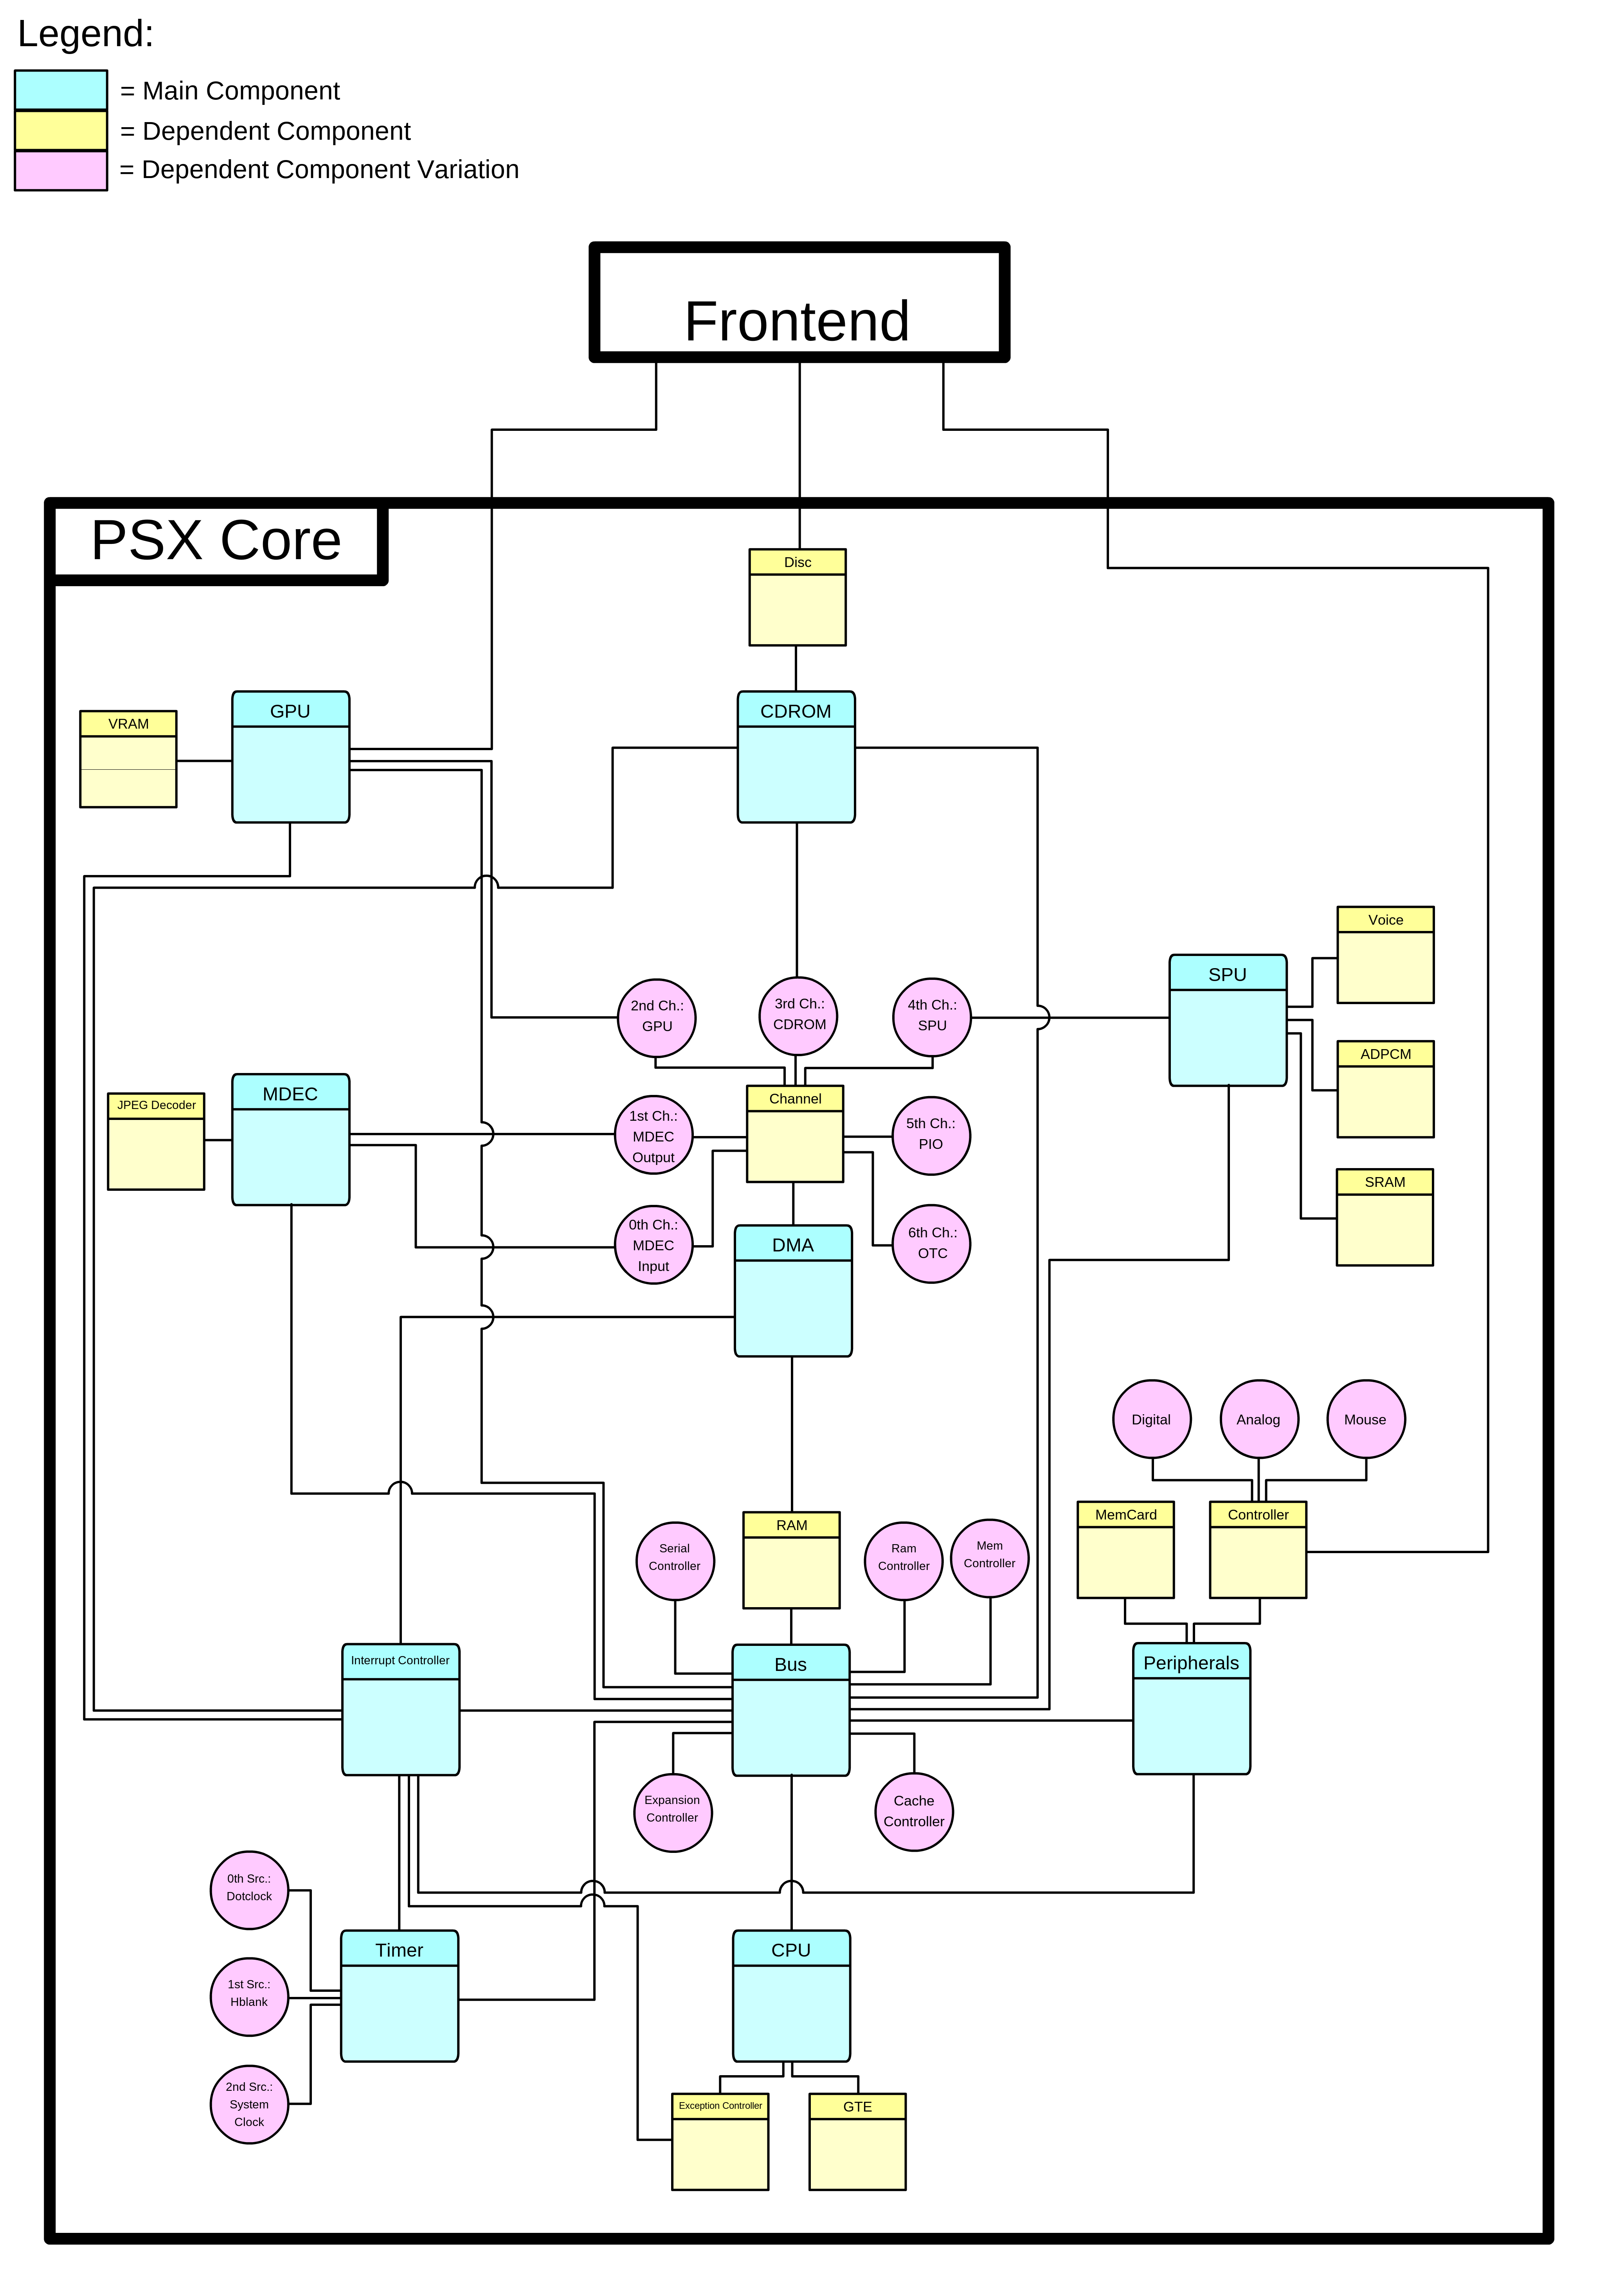
\includegraphics[width=1.0\textwidth]{obrazky-figures/psx-arch-simple.png}
\caption[Návrh architektury jádra emulátoru]{Kompletní návrh zapojení nejen hardwarových komponent emulátoru, ale i nadstavby nutné pro zpřístupnění stavu konzole.}
\label{psx-layout}
\end{figure}

\begin{figure}[hbt]
\centering
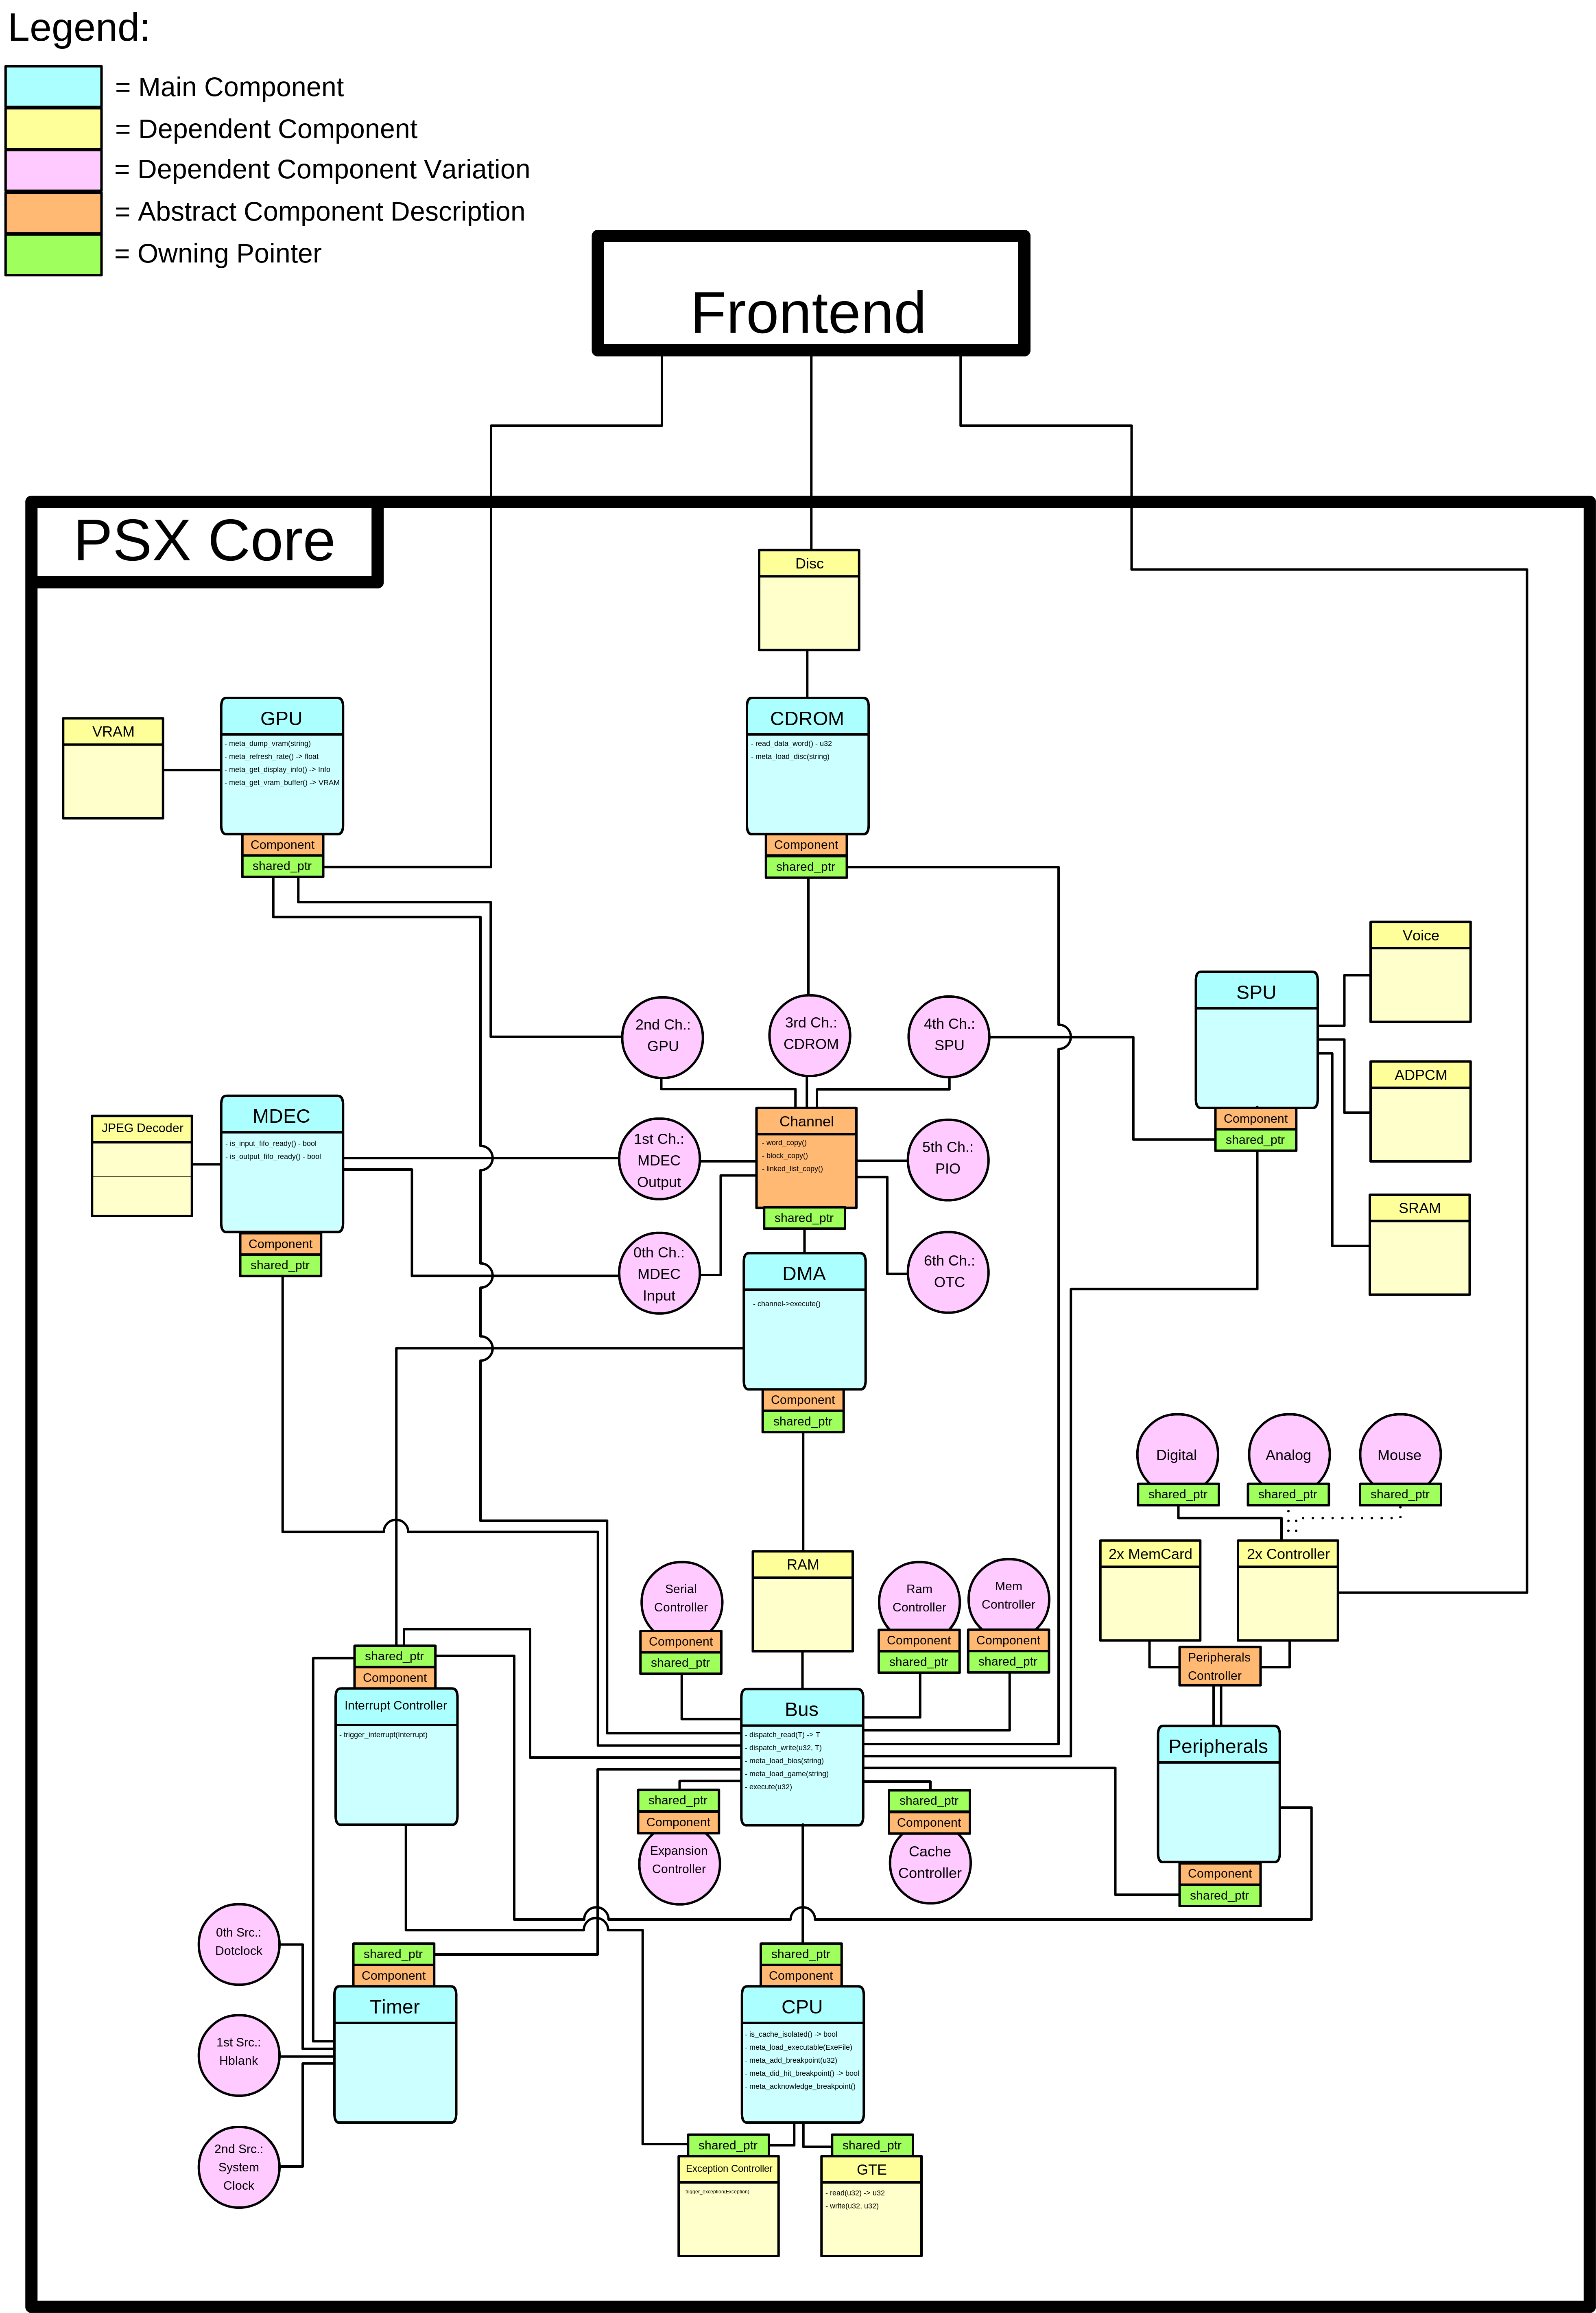
\includegraphics[width=1.0\textwidth]{obrazky-figures/psx-arch-detailed.png}
\caption[Detailní návrh architektury jádra emulátoru]{Povšimněme si, že každá komponenta dědí z generické virtuální třídy \textit{Component} \ref{component}, která je spravována přes \textit{smart} ukazatel.
To pak umožňuje jednoduše sdílet ten samý objekt mezi vícero komponentami.}
\label{psx-layout-detailed}
\end{figure}